\section{Interval model}
\label{sec:model}

Following the SQL:2011
standard~\cite{DBLP:journals/sigmod/KulkarniM12}, we adopt the {\em
  closed-open} period model, where a period (or interval) represents a
continuous set of time instances, starting from and including the
start time, continuing to but excluding the end time.  Time instances,
or chronons, have limited precision and the time domain $\omega_T$ is
linearly ordered and discrete.

\vspace{-0.2cm}
\begin{definition}[Time period]
A {\em time period} \\$p = [t_s, t_e)$ is an interval of the
  discrete time domain $\in \omega_T x \omega_T$, subject to the
  constraint $t_s < t_e$.
\label{def:period} 
\vspace{-0.2cm}
\end{definition}

We quantify relationships between time periods using the following
Allen's relations~\cite{allen83} with equality: \predName{meets},
\predName{overlaps}, \predName{starts}, \predName{finishes},
\predName{during}, and \predName{equals}.  We will use
$\pred{p}{contains}{q}$ as a shorthand for $\pred{p}{starts}{q} \vee
\pred{p}{finishes}{q} \vee \pred{p}{during}{q} \vee
\pred{p}{equal}{q}$.  We denote by $p \cap q$ the intersection of $p$
and $q$. \eat{$$to denote $[\predName{max}(p.start,q.start),
    \predName{min}(p.end, q.end))$.}\eat{ If
    $\predName{max}(p.start,q.start) \geq \predName{min}(p.end,
    q.end)$, then $p \cap q = \emptyset$.}

\begin{figure}
\centering
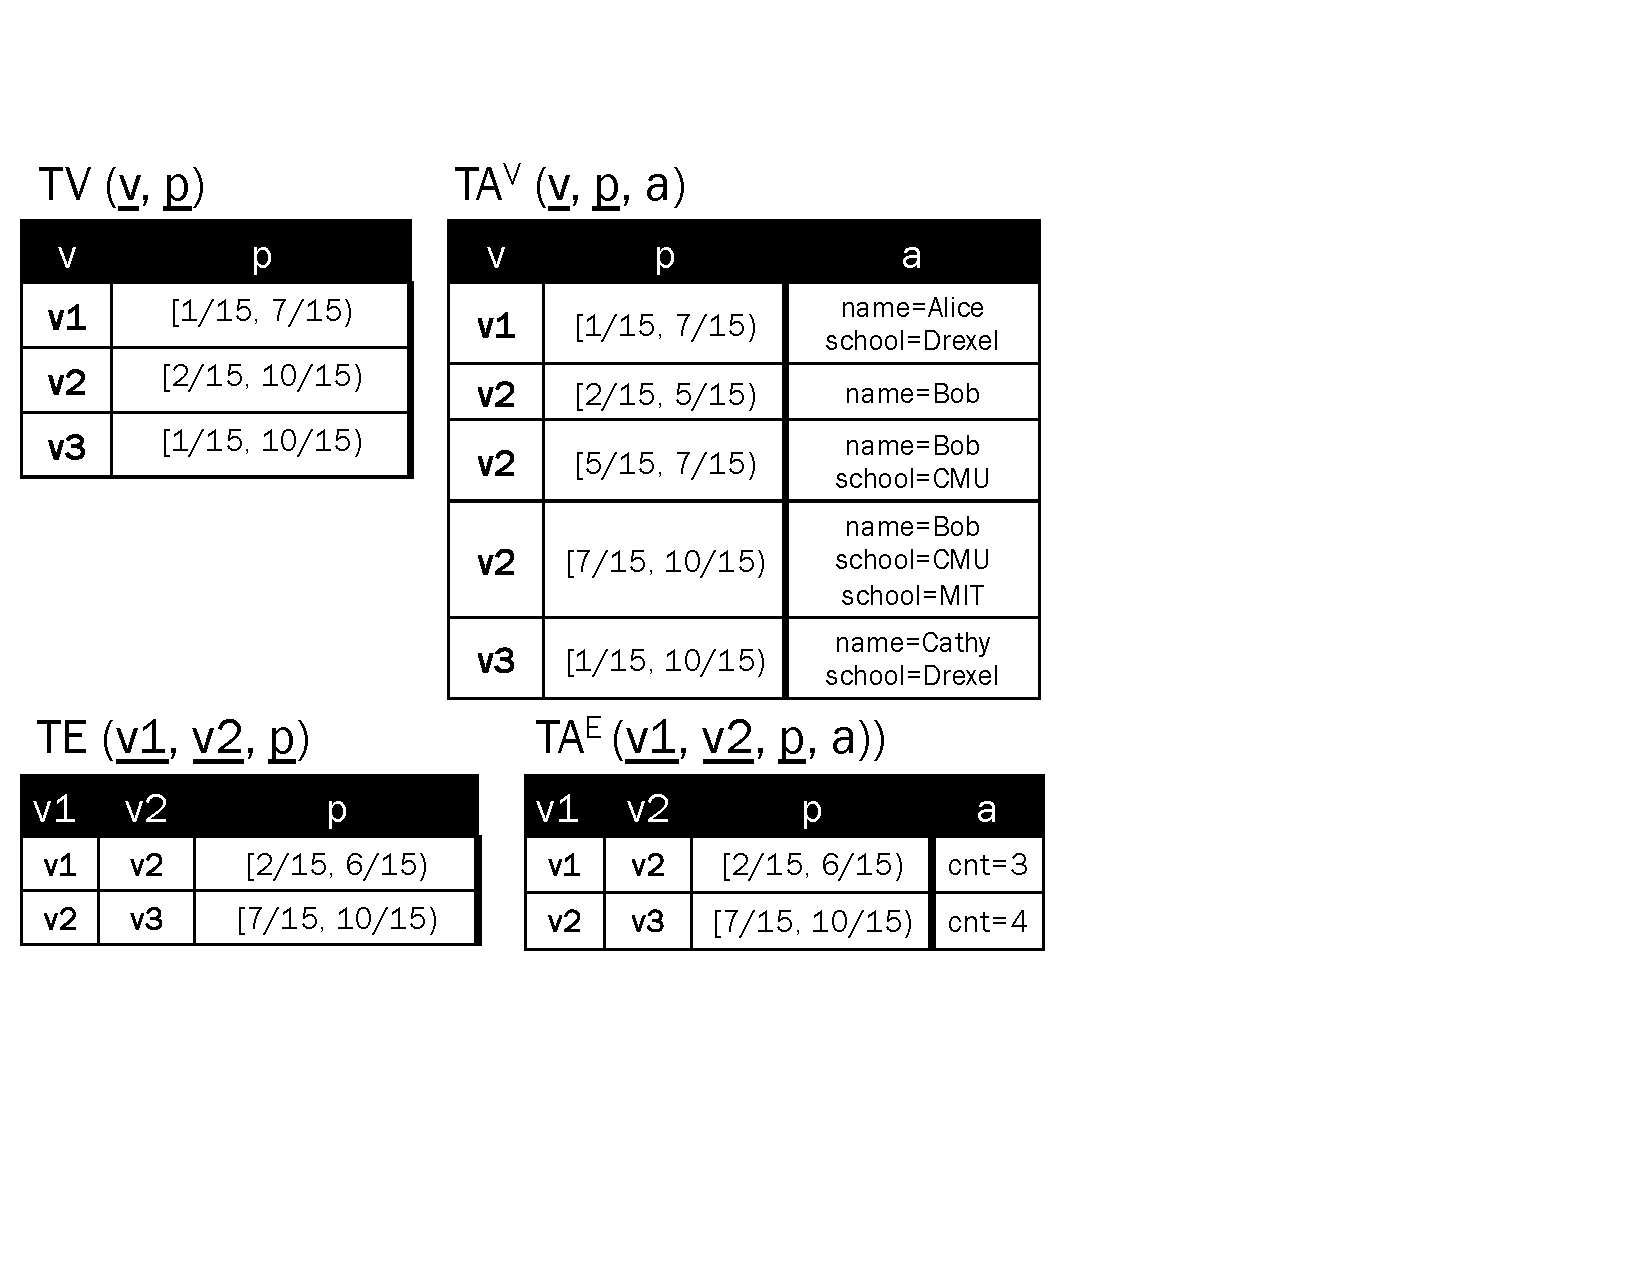
\includegraphics[width=3in]{figs/T1_rel.pdf}
\vspace{-0.2cm}
\caption{Vertex-edge representation.}
\vspace{-0.3cm}
\label{fig:tg_ve}
\end{figure}

We now give a representation of a \tg that uses valid-time temporal
SQL relations~\cite{DBLP:conf/vldb/BohlenSS96}, with nesting, to
represent evolution of graph topology and of its vertex and edge
attributes.  We term this logical representation the {\em \ve \tg}.
An example \ve \tg, representing evolving graph in
Section~\ref{sec:intro} is given in Figure~\ref{fig:tg_ve}.  Contrast
it with Figure~\ref{fig:coalesced}.

\vspace{-0.2cm}
\begin{definition}[Vertex-Edge TGraph]
A vertex-\\edge representation of \tg is a pair $\tve=(\tv, \te)$. \tv
is a valid-time temporal SQL relation with schema $\tv(\underline{v},
\underline{p})$ that associates a vertex with the time period during
which it is present. \te is a valid-time temporal SQL relation with
schema $\te(\underline{v_1}, \underline{v_2}, \underline{p})$,
connecting pairs of vertices from \tv.\eat{ Attribute $p$ represents
  time period (as per Definition~\ref{def:period}).} \tv and \te are
temporally coalesced:
\vspace{-0.3cm}
\begin{multline}
\vspace{-0.3cm}
\forall \tv(v, p)~~\nexists \tv(v, p')~~| \\
                       \pred{p}{meets}{p'}~\lor~\pred{p}{contains}{p'}~\lor~\pred{p}{overlaps}{p'}
\label{def:tg:c2}
\end{multline}
\vspace{-0.7cm}
\begin{multline}
\forall \te(v_1, v_2, p)~~\nexists \te(v_1,v_2, p')~~| \\
                       \pred{p}{meets}{p'}~\lor~\pred{p}{contains}{p'}~\lor~\pred{p}{overlaps}{p'}
\label{def:tg:c3}
\end{multline}

An edge connects a pair of vertices that exist at the time when the edge exists:
\vspace{-0.3cm}
\begin{multline}
\forall \te(v_1, v_2, p)~~\exists \tv(v_1, p_1), \tv(v_2, p_2)~~| \\
                       \pred{p_1}{contains}{p}~\wedge~\pred{p_2}{contains}{p}
\label{def:tg:c1}
\end{multline}
\vspace{-0.5cm}

\tve optionally includes vertex and edge attribute relations \tav
and \tae.  Both are coalesced, and associate bags of properties with
existing vertices and edges.
\vspace{-0.3cm}
\begin{multline}
\forall \tav(v, p, a)~~\nexists \tav(v, p', a)~~| \\
                       \pred{p}{meets}{p'}~\lor~\pred{p}{contains}{p'}~\lor~\pred{p}{overlaps}{p'}
\label{def:tg:c4}
\end{multline}
\vspace{-0.5cm}
\begin{multline}
\forall \tav(v, p, a)~~\exists \tv(v,p')~~|~~\pred{p'}{contains}{p}
\label{def:tg:c5}
\end{multline}
\vspace{-0.5cm}
\begin{multline}
\forall \tae(v_1, v_2, p, a)~~\nexists \tae(v_1, v_2, p', a)~~| \\
                       \pred{p}{meets}{p'}~\lor~\pred{p}{contains}{p'}~\lor~\pred{p}{overlaps}{p'}
\label{def:tg:c6}
\end{multline}
\vspace{-0.5cm}
\begin{multline}
\forall \tae(v_1, v_2, p, a)~~\exists \te(v_1,v_2,p')~~|~~\pred{p'}{contains}{p}
\label{def:tg:c7}
\end{multline}
\vspace{-0.6cm}
\label{def:tg}
\end{definition}
\vspace{-0.3cm}
Graphs may be directed or undirected.  For undirected graphs we choose
a canonical representation of an edge, with $v_1 \leq v_2$ (self-loops
are allowed).

Conditions~\ref{def:tg:c2} and~\ref{def:tg:c3} in
Definition~\ref{def:tg} state that \tv and \te are
coalesced~\cite{DBLP:conf/vldb/BohlenSS96}, i.e., that each vertex and
edge is represented exactly once for each time period of maximal
length when it is present.  Conditions~\ref{def:tg:c4}
and~\ref{def:tg:c6} state that all attribute relations are coalesced,
i.e., that an attribute is represented exactly once for each time
period of maximal length in which its value did not change.  Consider
Figure~\ref{fig:tg_ve} and note that there is a single tuple for $v_2$
in \tv, but three tuples for $v_2$ in \tav, because $school=CMU$ was
added at time 5/15, and $school=MIT$ at 7/15.  It is not required that
a vertex or an edge be represented in \tav and \tae --- a vertex or
edge that never had any associated properties will have no
corresponding tuples in \tav or \tae.

While our \ve representation is based on temporal SQL, we reiterate
that non-key attributes of vertices and edges are stored as
collections of properties.  Definition~\ref{def:tg} presents a logical
data structure and may be implemented, e.g., by a columnar
representation of vertex and edge properties (each property in a
separate relation), or by some hybrid representation.  A columnar
representation may be more efficient if different properties change at
different rates.

